\documentclass[a4paper,12pt]{article}
\usepackage[utf8]{inputenc}
\usepackage[T2A]{fontenc}
\usepackage[russian]{babel}
\usepackage{amsmath, amssymb, amsfonts, amsthm}
\usepackage{graphicx}
\usepackage{geometry}
\usepackage{float}
\usepackage[hidelinks, pdfencoding=auto, psdextra]{hyperref}
\usepackage{tocloft}
\usepackage{fancyhdr}
\usepackage{enumitem}
\usepackage{listings}
\usepackage{xcolor}
\usepackage{subcaption}

\geometry{top=2cm, bottom=2cm, left=2.5cm, right=2cm}
\setlength{\headheight}{14.5pt}

\begin{document}

\begin{titlepage}
    \centering
    {\Large \bfseries Федеральное государственное автономное образовательное учреждение высшего образования «Национальный исследовательский университет ИТМО» \par}
    
    {\large Факультет программной инженерии и компьютерной техники \par}
    \vspace{2cm}
    {\LARGE Домашнее задание №3 \par}
    \vspace{0.5cm}
    {\Large Вариант 74 \par}
    \vspace{2cm}
    \vfill
    \begin{flushright}
        \large
        \textbf{Выполнил:} \\
        Шулай Роман \\
        Группа P3115 \\
        \vspace{1cm}
        \textbf{Преподаватель:} \\
        Поляков Владимир Иванович \\
    \end{flushright}
    \vfill
    {\large Санкт-Петербург \\ 2026 год}
\end{titlepage}
\newpage
\setcounter{page}{2}

\begin{figure}[htbp]
    \centering
    \begin{subfigure}[b]{0.45\textwidth}
        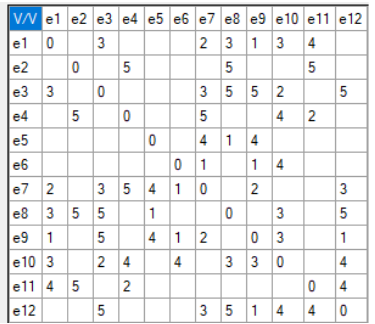
\includegraphics[width=\linewidth]{images/matrix.png}
        \caption{Матрица смежности}
        \label{fig:sub1}
    \end{subfigure}
    \hfill % Распорка для равномерного распределения
    \begin{subfigure}[b]{0.45\textwidth}
        
\includegraphics[width=\linewidth]{images/graph.png}
        \caption{Граф}
        \label{fig:sub2}
    \end{subfigure}
    %\caption{Общая подпись для двух картинок}
    \label{fig:main}
\end{figure}
\noindent
1. Пусть $s - e_1$, $t - e_{12}$ \\
2. Проведем разрез $K_1 = (\{s\},X\backslash\{s\})$ \\

\begin{figure}[H]
    \centering
    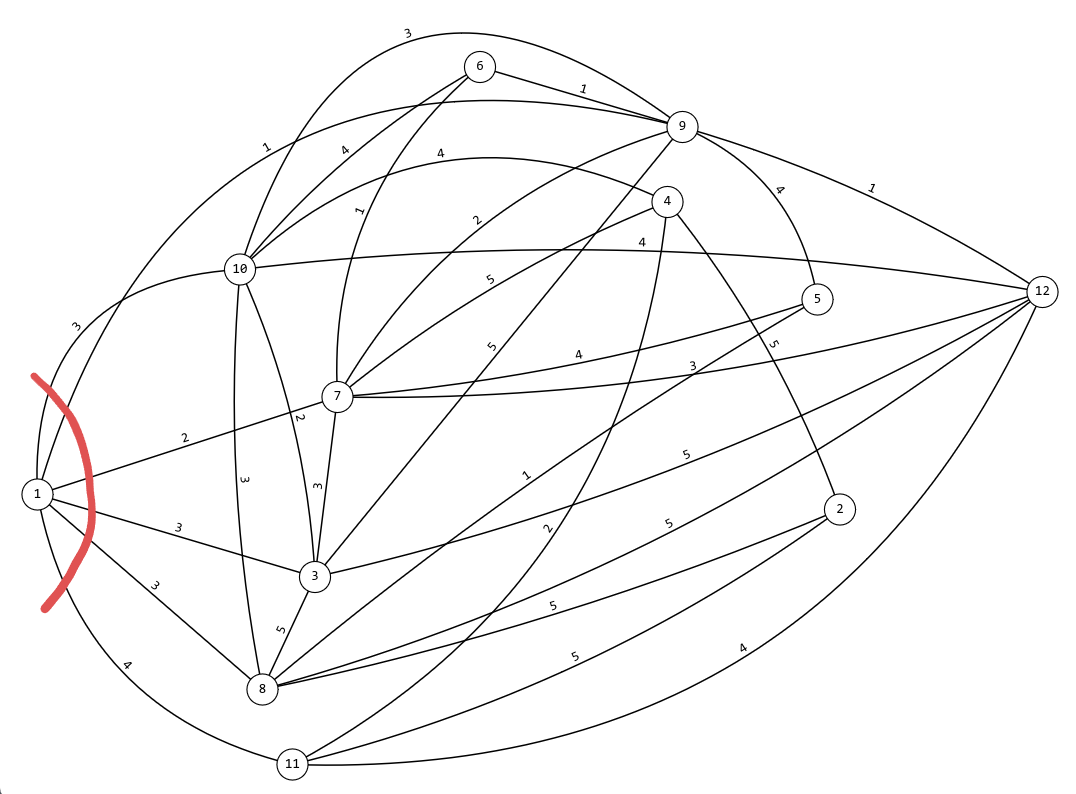
\includegraphics[width=0.7\linewidth]{images/3/step1color.png}
    \caption*{Разрез $K_1$}
\end{figure}
\noindent
3. Находим $Q_1 = max[q_{ij}] = 5$ \\
4. Закорачиваем все ребра графа $(e_i,e_j)$ с $q_{ij} \ge Q_1$. Это ребра $(e_2, e_8)$, $(e_2, e_{11}), (e_3, e_8)$, $(e_3, e_9)$, $(e_3, e_{12})$, $(e_4, e_7)$ и $(e_8, e_{12})$. Получаем граф $G_1$ \\
5. Проведем разрез $K_2$ \\

\begin{figure}[H]
    \centering
    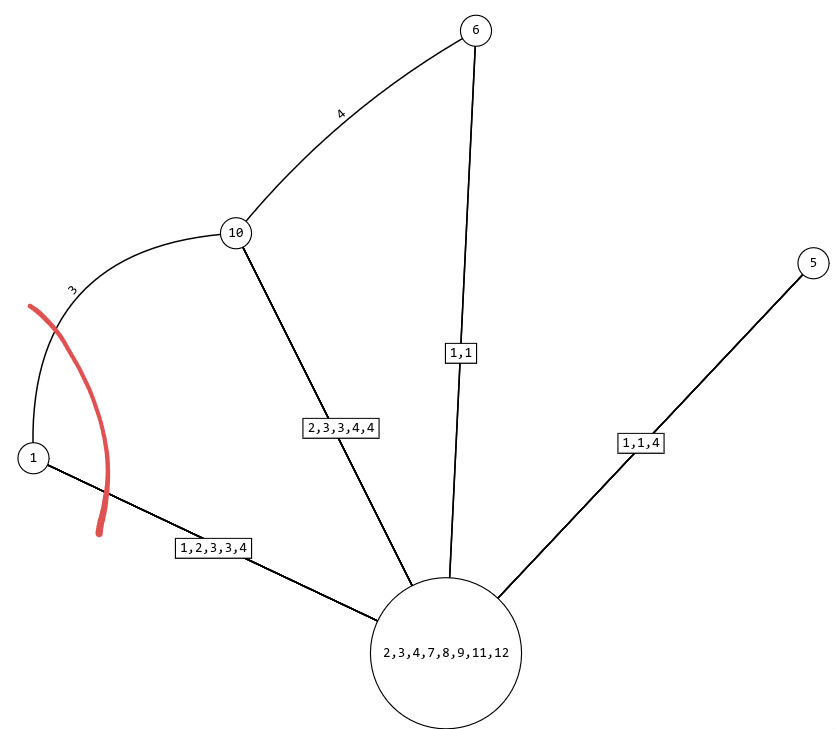
\includegraphics[width=0.7\linewidth]{images/3/step2color.png}
    \caption*{Разрез $K_2$}
\end{figure}
\noindent
6. Находим $Q_2 = max[q_{ij}] = 4$ \\
7. Закорачиваем все ребра графа $(e_i,e_j)$ с $q_{ij} \ge Q_2$. Получаем граф $G_2$

\begin{figure}[H]
    \centering
    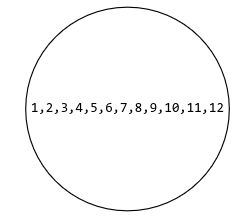
\includegraphics[width=0.4\linewidth]{images/3/step3.png}
    \caption*{Граф $G_2$}
\end{figure}
\noindent
8. Вершины $s$ и $t$ объединены. Пропускная способность искомого пути $Q(P)=4$ \\
9. Построим граф, вершины которого - вершины исходного графа, а ребра - ребра с пропускной способностью больше либо равной 4.

\begin{figure}[H]
    \centering
    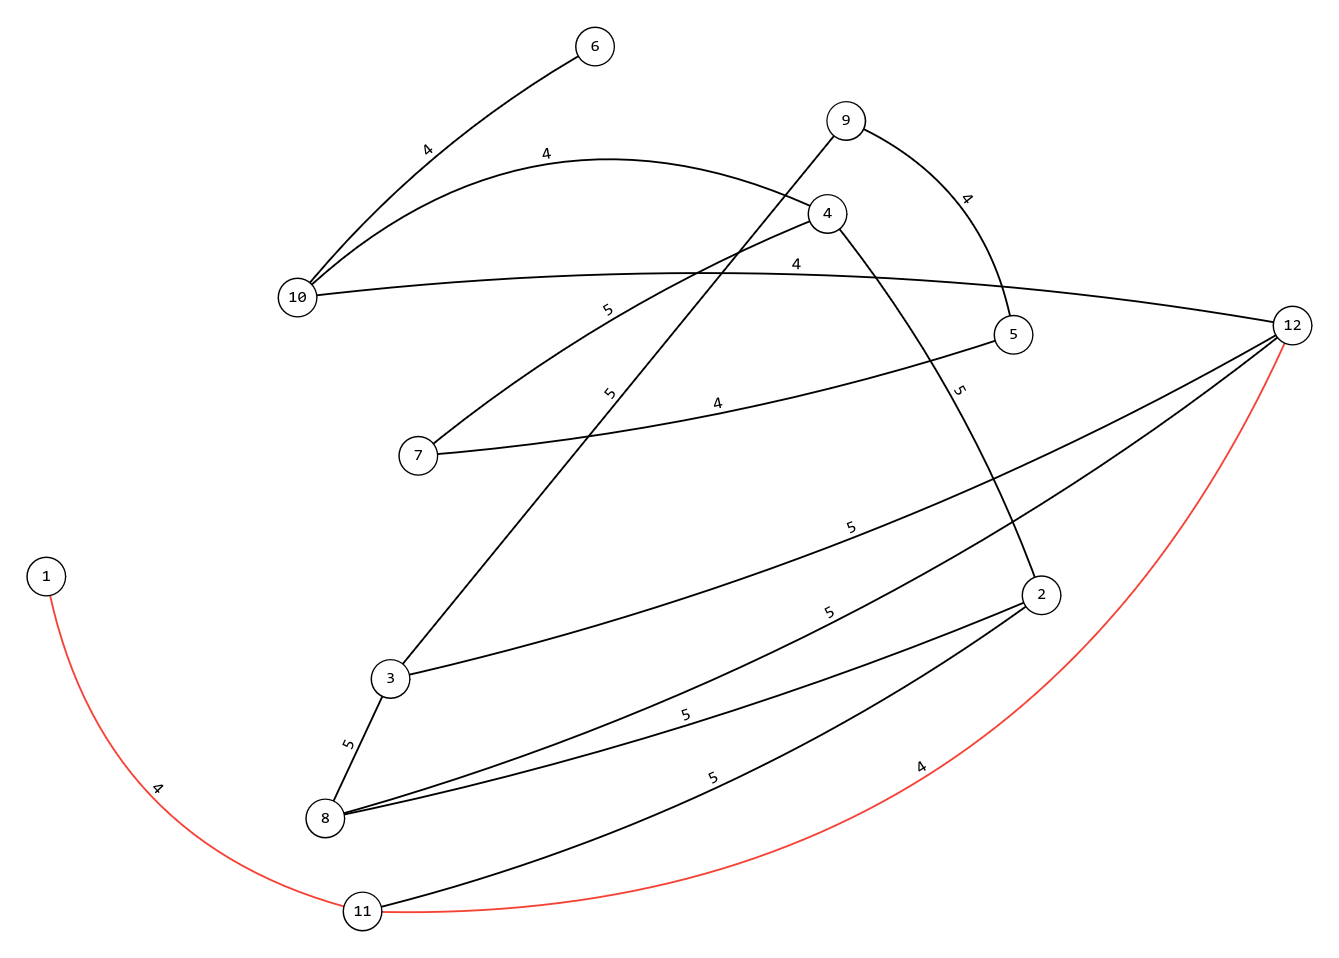
\includegraphics[width=0.7\linewidth]{images/3/final.png}
    \caption*{Путь с наибольшей пропускной способностью}
\end{figure}

\end{document}